% Appendix: sections after \appendix are numbered A, B, C, ...
\section{Source Code}\label{app:source_code}
The source code is available on \href{https://github.com/HuberNicolas/gaia-classifier}{GitHub}.

\section{Data}\label{app:data}

\subsection{Feature Subsets}

% Table with symbols, ticks and crosses, and a note below the rules
\begin{table}[H]
    \centering
    \begin{tabular}{lrrcc}
        \toprule
        \textbf{Dataset} & \textbf{Size} & \textbf{Accuracy} & \textbf{Symbol} & \textbf{Used} \\
        \midrule
        Dataset A & 1000 & 92\,\% & $\dagger$ & \ding{51} \\
        Dataset B & 5000 & 87\,\% & $x$       & \ding{55} \\
        Dataset C & 2000 & 95\,\% & $o$       & \ding{51} \\
        \bottomrule
        \multicolumn{5}{l}{\footnotesize $\dagger$: Symbol A, $x$: Symbol B, $o$: Symbol C} \\
    \end{tabular}
    \caption{Summary of datasets and accuracy}
    \label{tab:datasets}
\end{table}

\section{Evaluation}\label{app:evaluation}

\begin{figure}[H]
    \centering
    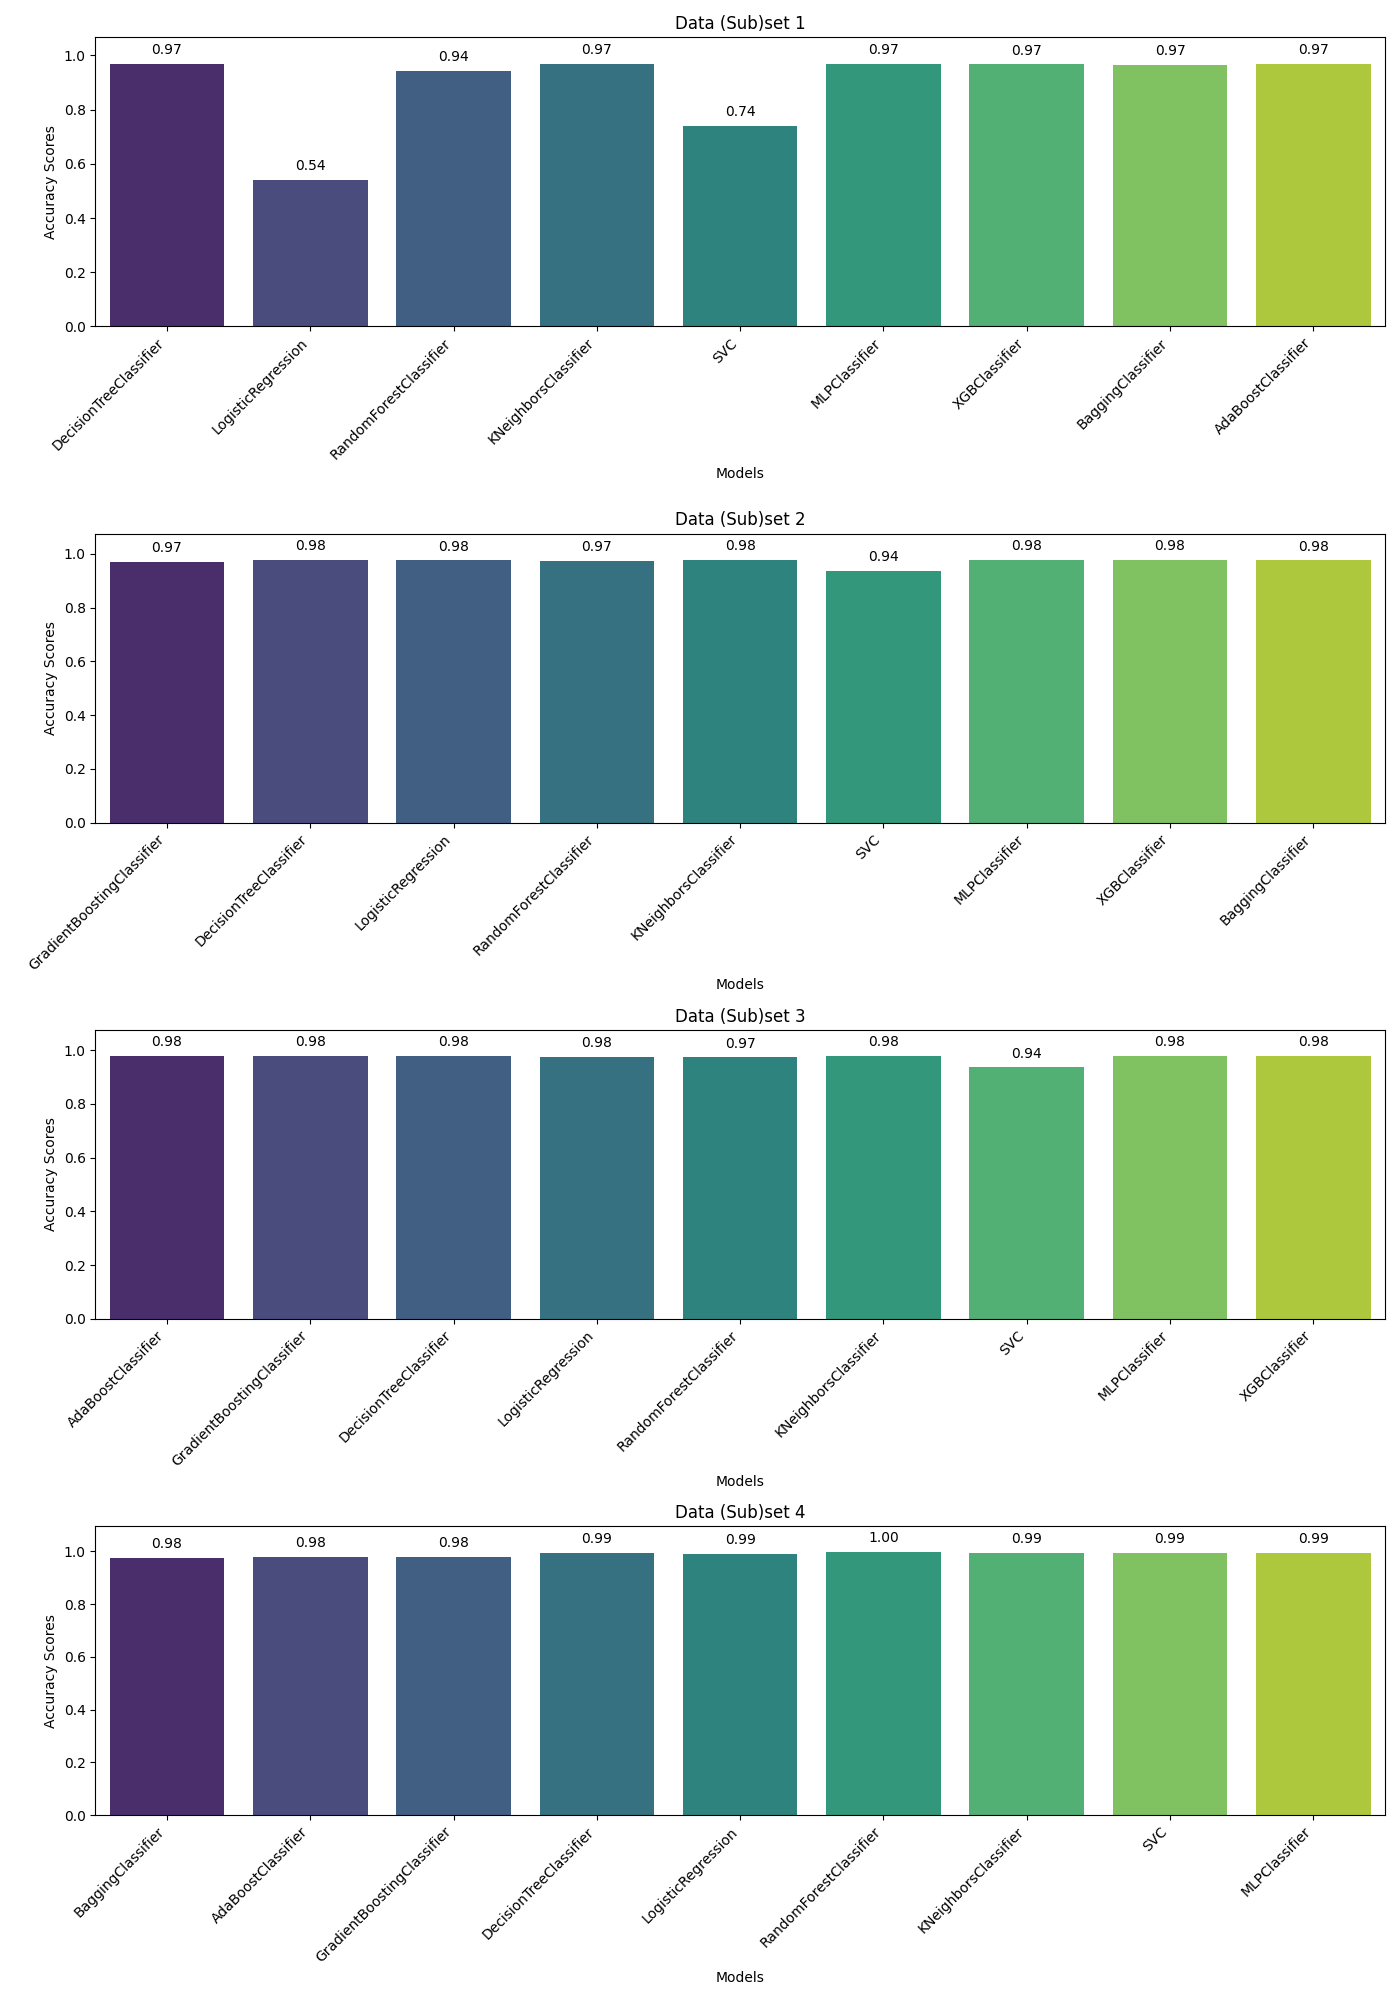
\includegraphics[width=0.8\linewidth]{assets/images/best_classifier/50_data_eval.png}
    \caption{Accuracy of the models on the feature subsets (50\,\% of the training data)}
    \label{fig:eval_bar_scores_50}
\end{figure}

\subsection{Metrics for the Best Model}\label{app:metrics}

% Matrix and aligned equations
Based on the confusion matrix
\[
    \begin{bmatrix}
        15950 & 47 \\
        35    & 13676
    \end{bmatrix},
\]
the metrics are:
\begin{align*}
    \text{Accuracy}    &= \frac{TP + TN}{TP + TN + FP + FN} = \frac{13676 + 15950}{13676 + 15950 + 47 + 35} = \frac{29626}{29708} \approx 0.9972 \\
    \text{Precision}   &= \frac{TP}{TP + FP} = \frac{13676}{13676 + 47} = \frac{13676}{13723} \approx 0.9966 \\
    \text{Recall}      &= \frac{TP}{TP + FN} = \frac{13676}{13676 + 35} = \frac{13676}{13711} \approx 0.9974 \\
    \text{Specificity} &= \frac{TN}{TN + FP} = \frac{15950}{15950 + 47} = \frac{15950}{15997} \approx 0.9971 \\
    \text{F1 score}    &= 2 \cdot \frac{\text{Precision} \cdot \text{Recall}}{\text{Precision} + \text{Recall}} \approx 0.9970 \\
    \text{FPR}         &= \frac{FP}{FP + TN} = \frac{47}{15997} \approx 0.0029 \\
    \text{FNR}         &= \frac{FN}{FN + TP} = \frac{35}{13711} \approx 0.0026 \\
    \text{FDR}         &= \frac{FP}{TP + FP} = \frac{47}{13723} \approx 0.0034
\end{align*}
